%\section{Introduction}
\chapter{Introduction}\label{cha:Introduction}
The development and research of compressed sensing applied to a single pixel camera (SPC) is a relatively new area in signal processing with the first functioning camera architecture in 2006. Since then numerous improvements and methods have been proposed on how to capture images. In this section an introduction to the SPC architecture and a brief introduction to compressed imaging (CI) is presented followed by the aim, research questions and thesis outline. 



%\subsection{Background}
\section{Background}
Compressed sensing (CS) allows reconstruction of a sparse signal being sampled with far fewer samples required to fulfill the sampling theorem. Swedish Defence Research Agency (FOI) became interested in the subject some years ago and tests potential applications. One of the potential applications are a camera with a single pixel which can reconstruct a scene, therefore FOI built a SPC platform in the short-wave infrared (SWIR) spectrum for the purpouse to study and evaluate this kind of system.\\[0.1in]

The SWIR spectrum is electromagnetic radiation with wavelengths between 700 - 2500 nm and SWIR cameras can therefore capture images illuminated by the sun, moon, starlight and airglow that works both at day and night. SWIR light can to some extent pass through smoke and fog which makes it a robust camera for day and night applications. Some camouflage that is hard to spot in visual spectrum is visible in the SWIR spectrum. The system used in this master’s thesis uses a digital micromirror device (DMD) to sample the light from the scene. The system will sample less single pixel measurements than the number of pixels in the reconstructed image with the drawback that it has to capture each measurement in consecutive order instead of all at the same time.

%\subsection{Compressive sensing and imaging}
\section{Compressive sensing and imaging}
Compressive sensing is a new sampling strategy which reconstructs a compressible or sparse signal by finding a solution to an underdetermined linear system where the number of single pixel measurements is less than the number of pixels in the final reconstructed image. Two constraints need to be fulfilled to apply compressed sensing sampling: the sampled image needs to be sparse in some basis, e.g. the Fourier or wavelet base, and the measurement matrix must be incoherent with the sparse transform, meaning that the image needs to be compressible and the selected sampled pixels for each measurement needs to be picked at random with a 50\% chance of being included in the measurement.\cite{article:CS_donoho1} \\[0.1in]

The characteristic  underdetermined linear system in CS is defined as $ \mathbf{y} = \mathbf{\Phi}\mathbf{x}$, where $\mathbf{y}$ contains the measurements from the measurement matrix $\mathbf{\Phi}$ sensing the image $\mathbf{x}$. In figure~\ref{fig:CS_eq_sys} such a linear equation system is shown.

\begin{figure}[H]
	\centering
	\includegraphics[scale=0.5]{gfx/CS_eq.eps}
	\caption{The compressive sensing characteristic underdetermined linear system. The image $\mathbf{x}$ represented as a vector, being sampled with a measurement matrix $\mathbf{\phi}_m$ (one row of the complete measurement matrix $\mathbf{\Phi}$) yielding one measurement $\mathbf{y}_i$.}
	\label{fig:CS_eq_sys}
\end{figure}

The SPC in this master's thesis was designed with reflecting telescope optics to act as a lens to focus the scene. As seen in figure~\ref{fig:system_overview} light from the scene enters through the aperture in the camera where the primary mirror focus the light the via the secondary mirror onto the DMD. To this point, the SPC works like a conventional camera with a DMD where the image sensor would be placed in the convectional camera. The DMD resembles an image sensor, but instead of photo diodes for each pixel there is a tiny mirror which corresponds to one pixel and can individually either reflect the incoming light to the single pixel sensor being measured or reflect the light in the other direction without measuring it.


%SWIR is the short wave infrared spectrum and is defined in the wavelengths between 700 to 2500 nm just where humans perception of red wavelength ends SWIR starts.


\begin{figure}[H]
\centering
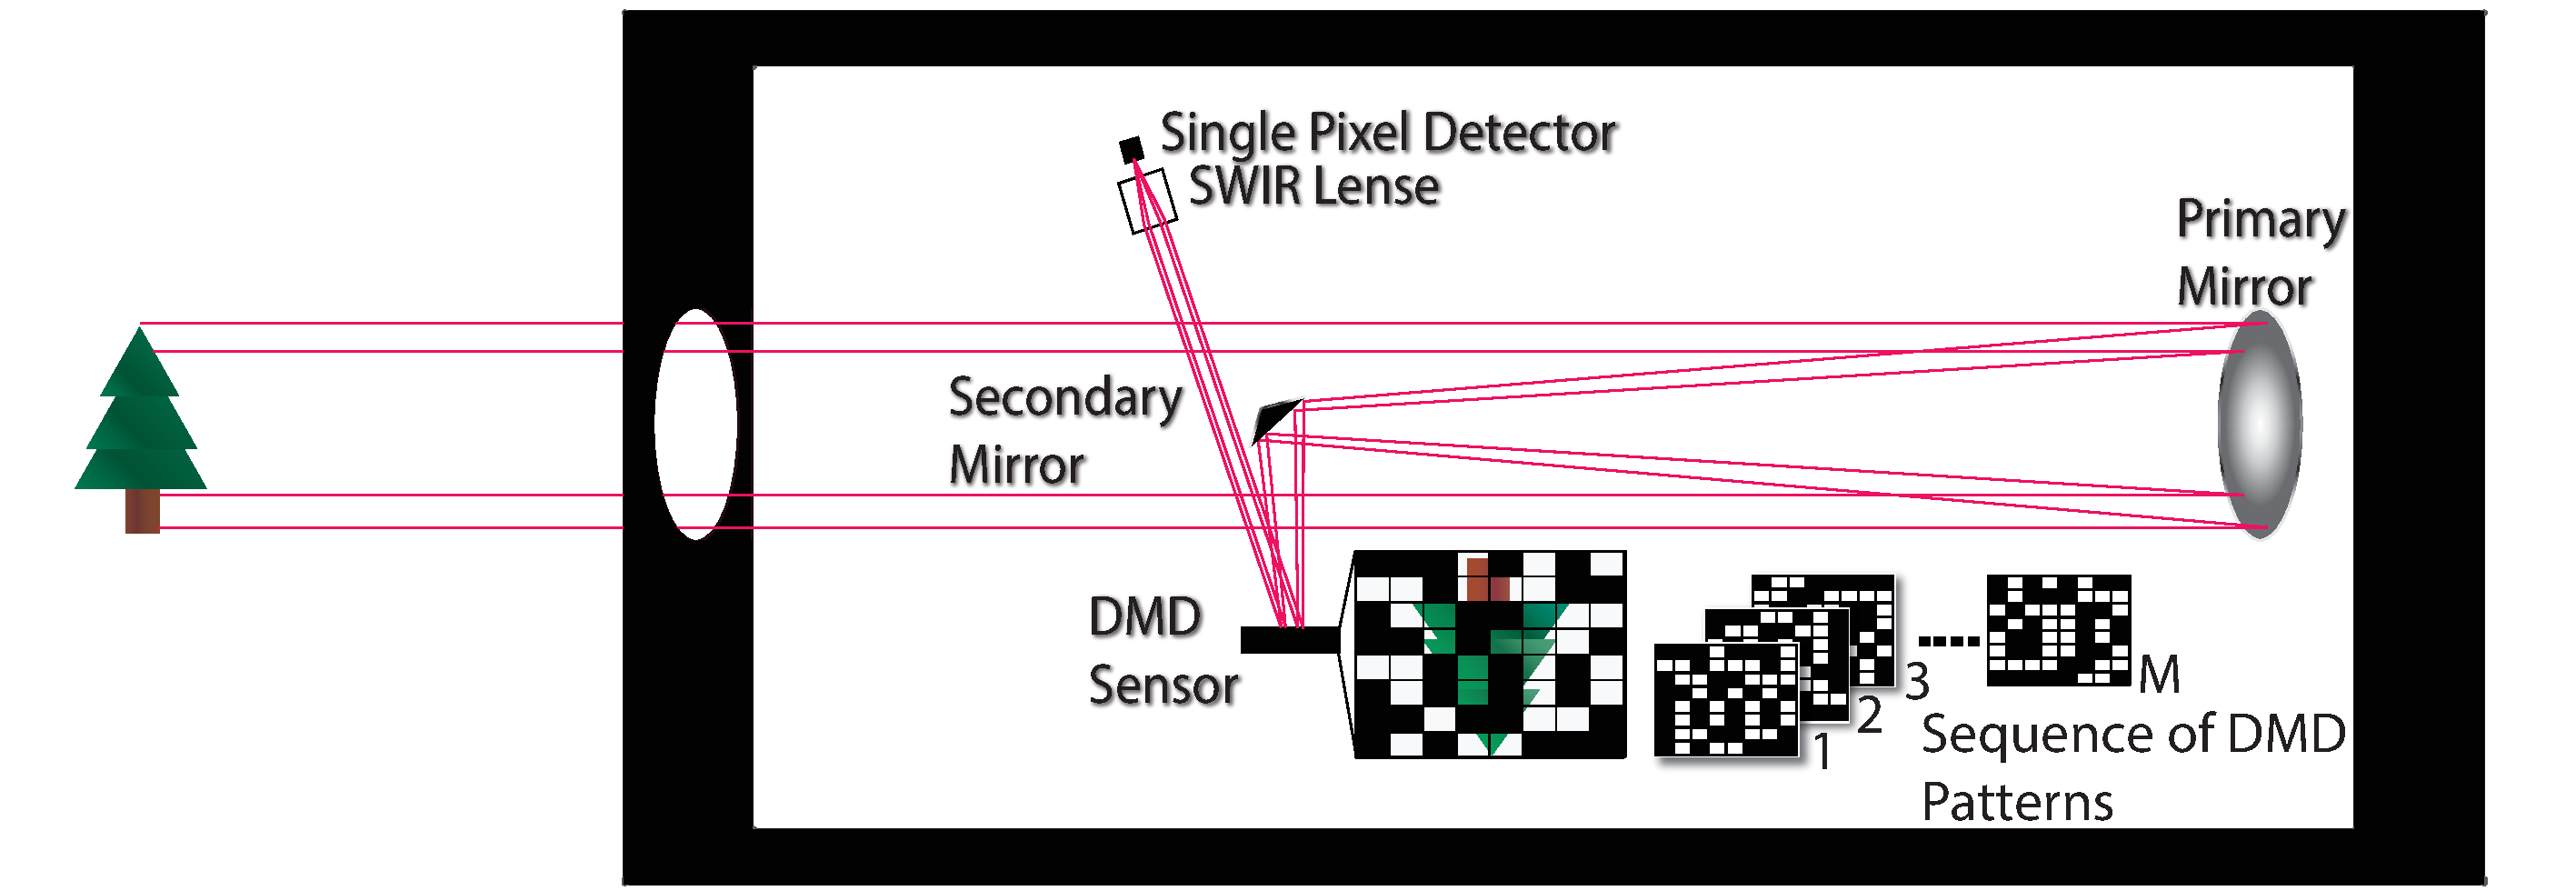
\includegraphics[width = \linewidth]{gfx/System_gif.eps}
	\caption{SPC system overview.}
	\label{fig:system_overview}
\end{figure}	

To connect the CS linear system in figure~\ref{fig:CS_eq_sys} to the single pixel camera each row of the complete measurement matrix is being re-sized to a square matrix of ones and zeros and displayed on the DMD as a pattern, which act as a filter for which pixels being sampled by the single pixel sensor. The next measurement is then performed by the next measurement matrix until all desired measurements are completed, as shown in figure~\ref{fig:system_overview}.\\[0.1in]

When all the measurements are sampled, an optimization algorithm calculates the most significant coefficients of the image in another more sparse basis, for example the wavelet basis, by transforming the complete measurement matrix. Because the image is more sparse or compressed in another basis, it is easier to find the solution to the equation system in that basis. Hence the name compressive sensing and the reason why the image can be reconstructed using less measurements than number of pixels.    

%Scientists at Rice university in Texas, USA realized that the new method could be used to create a new camera architecture with a single photo diode in the sensor, the single pixel camera was born and thus a new sub field of compressed sensing was created called compressive imaging.\\[0.1in] 






%To connect the architecture with the math from CS it can be interpreted as, the light from the scene which is focused on the DMD is the desired signal $\mathbf{x}$, the image. The DMD can individually set each mirror the ether direct the light from each mirror (image pixel) to the single pixel sensor or dump the light i.e a spatial light modulator (SLM). The DMD sets a pattern of pixel of intressed which is a measurement matrix $\Phi_m$ to be summarized in the single pixel sensor $y_m$ as a measurement. One measurement is the inner product of a measurement matrix and the signal, $\Phi_m \times x = y_m$. To complete a full measurement the process is repeated with different measurement matrices set on the DMD to the full underdetermined linear system $ \mathbf{y} = \mathbf{\Phi}\mathbf{x}$.


   

 
%\subsection{Motivation}
\section{Motivation}
Why would an SPC be beneficial to a conventional camera? The SPC has more components and several measurements have to be made over time, while a regular camera measures all pixels on the sensor at the same time. Moreover the reconstruction shifts burden to the processor. There are two major reasons why an SPC is of interest. The SPC can not compete with the conventional cameras in the visual spectrum where cameras in all price ranges and quality already exist and are relative cheap to build. The focus lies in more exotic spectra like SWIR or Terahertz (X-ray), where the image sensors are hard to build. This brings up cost and the ability to create high resolution sensors. With CS and the SPC architecture, manufacturing cost can be significantly reduced while the image resolution increases. For example, a state of the art SWIR camera cost about half a million SEK. The cost can be reduced by a factor of 20 or higher with an SPC with the same resolution. 

%\subsection{Aim} 
\section{Aim} 
\label{sec:aim}
What image quality can be achieved in natural images captured with a single pixel camera in daylight using state of the art methods?\\[0.1in]  

%Which resulted in three \textit{research questions} in support of finding the answer to the aim:

\section{Research questions} 
\label{sec:RQ}
\begin{itemize}
    \item How can the quality of images reconstructed by CS or a SPC be evaluated?
    \item What is the state of the art method to capture and reconstruct images using a SPC architecture?
    \item What image quality is achieved using state of the art methods applied to the SPC?
\end{itemize}

\section{Limitations}
\begin{itemize}
    \item The SPC provided by FOI is used and only minor changes can be made.
    \item The SPC is stationary at FOI and images can only be captured from the building.
    \item The reconstruction algorithm will not be developed in this thesis and therefore free to use algorithms needs to be found.
\end{itemize}



\section{Thesis outline}
In this thesis the most important and inspirational articles will be presented with a small description in section~\ref{sec:related_work} \textit{Related work}. Section~\ref{sec:method} \textit{Method} presents a thorough review of the hardware, sensing- and reconstruction-method and the complete image capturing chain including pre- and post-processing. The method section includes essential compressive sensing and imaging theory, this section also presents the evaluation techniques used in the result. Section~\ref{sec:Evaluation} \textit{Results} is divided into two categories, \textit{simulated results} and \textit{SPC results}, where the same evaluation technique is performed on simulated and SPC images respectively in order to draw conclusions of the different parts of the chain. The results are followed by \textit{Discussion} and \textit{Conclusion \& Future Work} in section~\ref{sec:discussion} and \ref{sec:conclusions_and_fw} respectively. 
